\documentclass[12pt, titlepage]{article}

\usepackage{fullpage} %full page typesetting
\usepackage{setspace} %allows for non-singlespacing
\usepackage{graphicx} %graphics capabilities
\usepackage{latexsym} %extra symbols
\usepackage{rotating} %rotation for figures
\usepackage{longtable} %tables that fill more than a single page
%\usepackage{hyperref} %hypertext links in the document
\usepackage{natbib} %better bibliographies
\usepackage{authblk} %author and affiliation in opening
\usepackage{mathpazo} %use palatino font, rather than times
\usepackage{appendix}
\usepackage{lscape}
\usepackage{tabulary}
\usepackage[nottoc]{tocbibind}
\usepackage[colorlinks=true,linkcolor=blue,citecolor=cyan]{hyperref}
\usepackage{ifthen}
\usepackage{float}
\usepackage{subcaption}
\usepackage{mwe}
\usepackage{caption}
\usepackage{listings}
\lstset{
	basicstyle=\small\ttfamily,
	columns=flexible,
	breaklines=true
}

\title{\tb{Place of Residence and Political Attitudes in Democracies Worldwide \\ {\large Online Appendix B -- Residual Plots} }}

\author{Jennifer Lin}
\affil{New College of Florida}

\newcommand\e{\emph}
\newcommand\tb{\textbf}
\newcommand\un{\underline}
\newcommand\txt{\texttt}

\doublespacing 

\begin{document}

\begin{singlespace}
\maketitle
\end{singlespace}

\section{Residual Plots for General Trends}

For the general model, the regressions that were ran used the following code:

\begin{lstlisting}
regress ideology i.place gender age education ses partyid closeness religion
regress liberalism i.place gender age education ses partyid closeness religion
\end{lstlisting}

The Residual versus Fitted plots for the models are as follows:

\begin{figure}[H]
	\centering
	\begin{subfigure}[b]{0.475\textwidth}   
		\centering 
		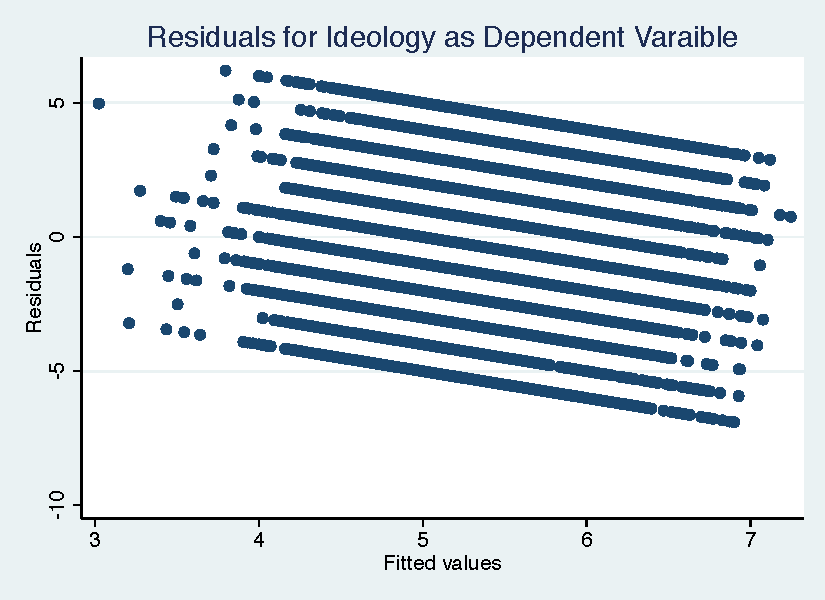
\includegraphics[width=\textwidth]{Residuals/ResidAllIdeo}
		\caption{Self-Placement Ideology}
	\end{subfigure}
	\hfill
	\begin{subfigure}[b]{0.475\textwidth}
		\centering 
		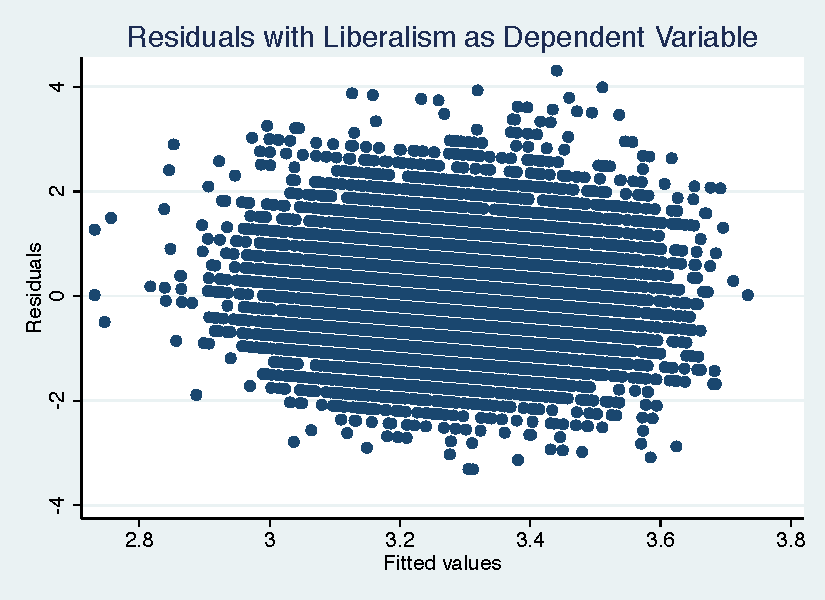
\includegraphics[width=\textwidth]{Residuals/ResidAllLib}
		\caption{Issue Stances}
	\end{subfigure}
	\caption{Residual Plots for Individual-Level Responses}
	\label{AllRVF}
\end{figure}

For the inclusion of all countries and their macro variables, the following regression commands are used:

\begin{lstlisting}
regress ideology i.place democracy electformula regimeage freedomhouse corruption gender age education ses partyid closeness religion
regress liberalism i.place democracy electformyla regimeage freedomhouse corruption gender age education ses partyid closeness religion
\end{lstlisting}

\begin{figure}[H]
	\centering
	\begin{subfigure}[b]{0.475\textwidth}   
		\centering 
		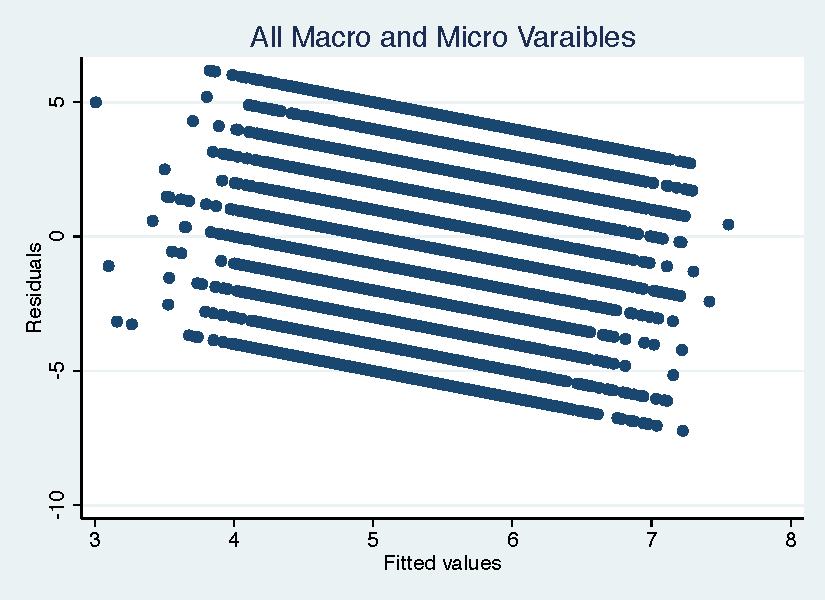
\includegraphics[width=\textwidth]{Residuals/Macroresid}
		\caption{Self-Placement Ideology}
	\end{subfigure}
	\hfill
	\begin{subfigure}[b]{0.475\textwidth}
		\centering 
		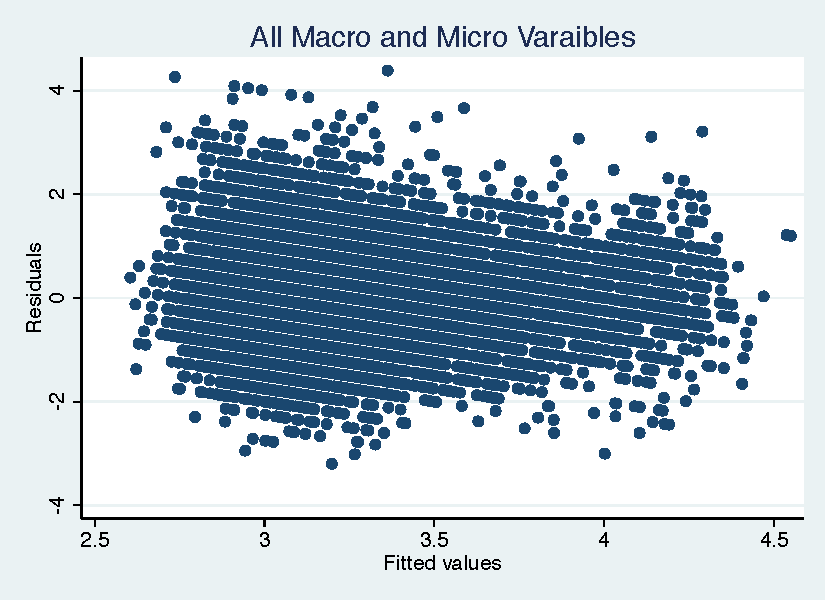
\includegraphics[width=\textwidth]{Residuals/Macroresidlib}
		\caption{Issue Stances}
	\end{subfigure}
	\caption{Residual Plots for Macro-Level Variables and Individual-Level Responses}
	\label{AllMacroRVF}
\end{figure}


\section{Residual Plots for Each Country}


\begin{figure}[H]
	\centering
	\begin{subfigure}[b]{0.475\textwidth}   
		\centering 
		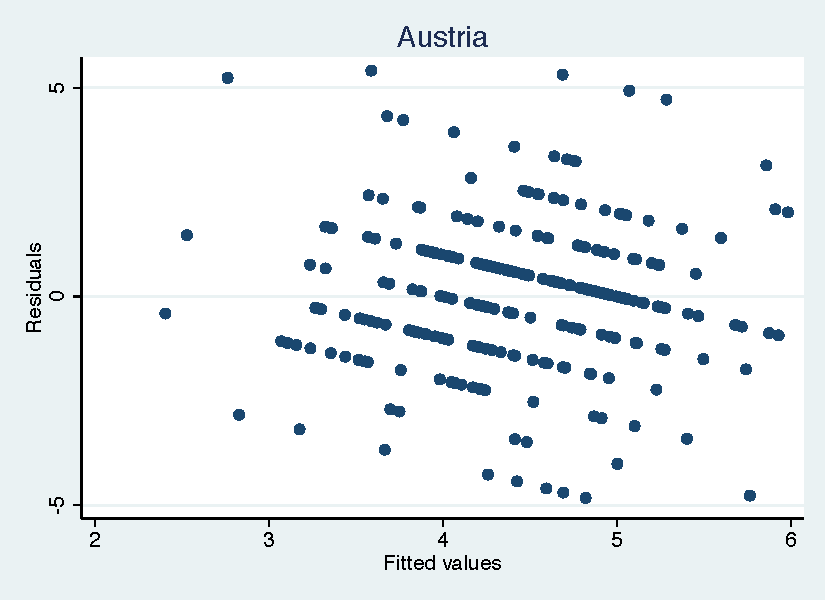
\includegraphics[width=\textwidth]{Residuals/CountryIdeo/Austria}
		\caption{Self-Placement Ideology}
	\end{subfigure}
	\hfill
	\begin{subfigure}[b]{0.475\textwidth}
		\centering 
		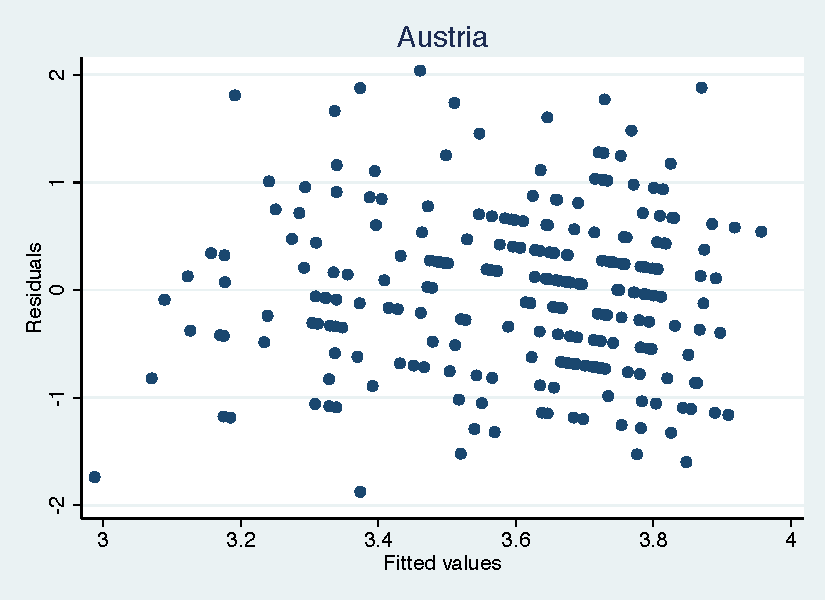
\includegraphics[width=\textwidth]{Residuals/CountryLib/Austria}
		\caption{Issue Stances}
	\end{subfigure}
	\caption{Austria}
	\label{Austria}
\end{figure}

\begin{figure}[H]
	\centering
	\begin{subfigure}[b]{0.475\textwidth}   
		\centering 
		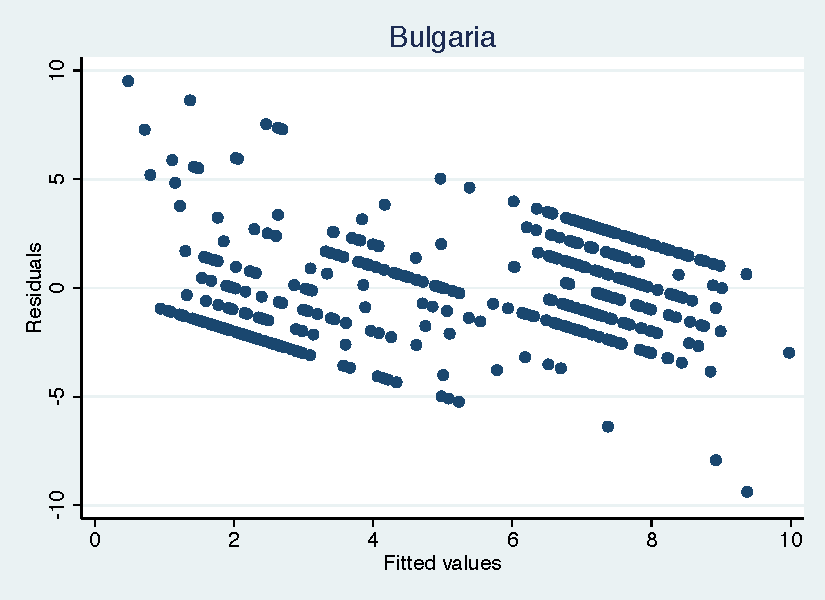
\includegraphics[width=\textwidth]{Residuals/CountryIdeo/Bulgaria}
		\caption{Self-Placement Ideology}
	\end{subfigure}
	\hfill
	\begin{subfigure}[b]{0.475\textwidth}
		\centering 
		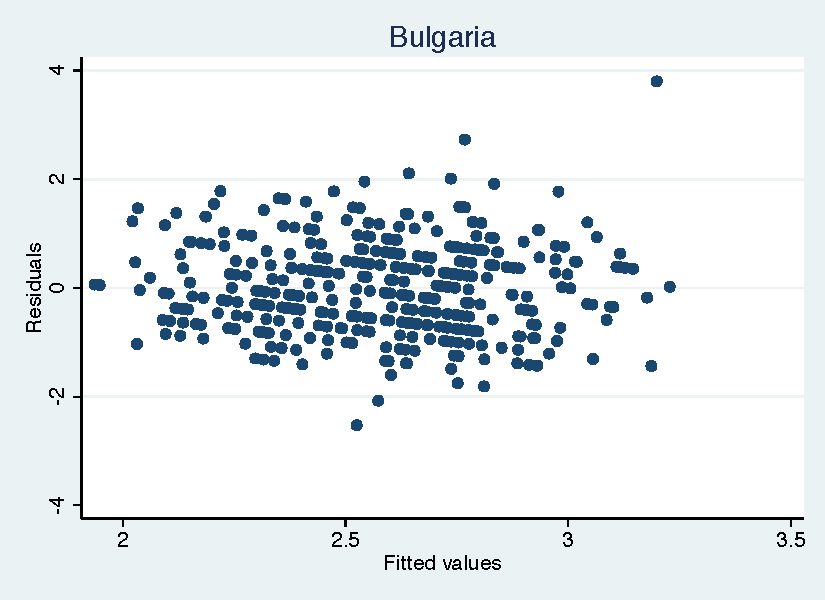
\includegraphics[width=\textwidth]{Residuals/CountryLib/Bulgaria}
		\caption{Issue Stances}
	\end{subfigure}
	\caption{Bulgaria}
	\label{Bulgaria}
\end{figure}

\begin{figure}[H]
	\centering
	\begin{subfigure}[b]{0.475\textwidth}   
		\centering 
		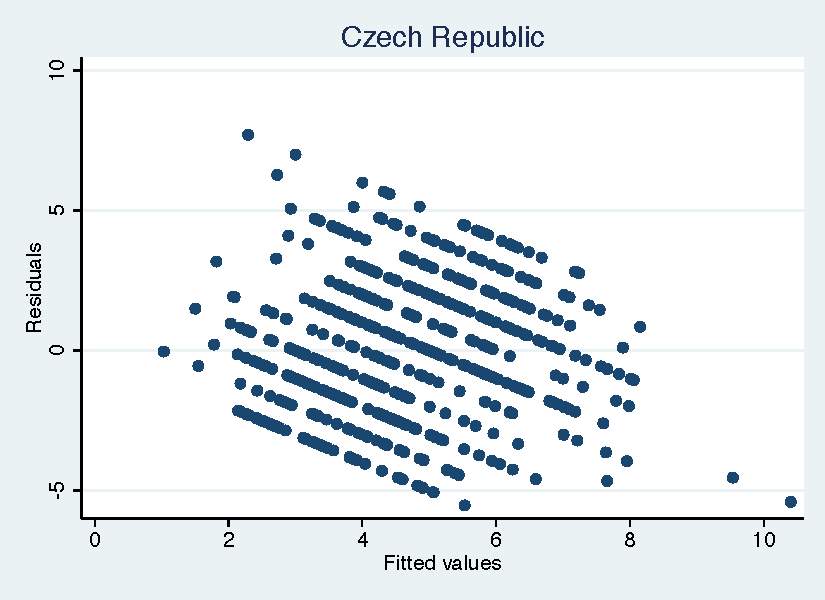
\includegraphics[width=\textwidth]{Residuals/CountryIdeo/Czech}
		\caption{Self-Placement Ideology}
	\end{subfigure}
	\hfill
	\begin{subfigure}[b]{0.475\textwidth}
		\centering 
		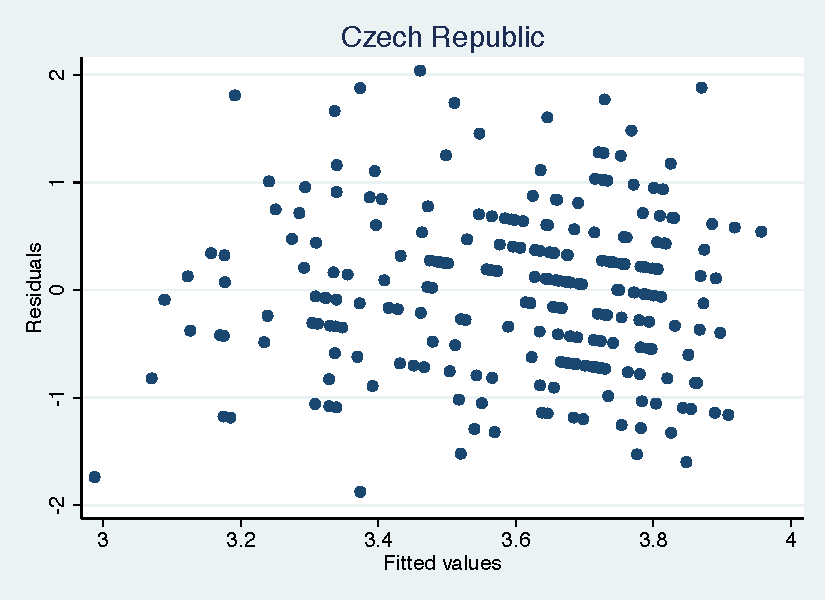
\includegraphics[width=\textwidth]{Residuals/CountryLib/Czech}
		\caption{Issue Stances}
	\end{subfigure}
	\caption{Czech Republic}
	\label{Czech}
\end{figure}

\begin{figure}[H]
	\centering
	\begin{subfigure}[b]{0.475\textwidth}   
		\centering 
		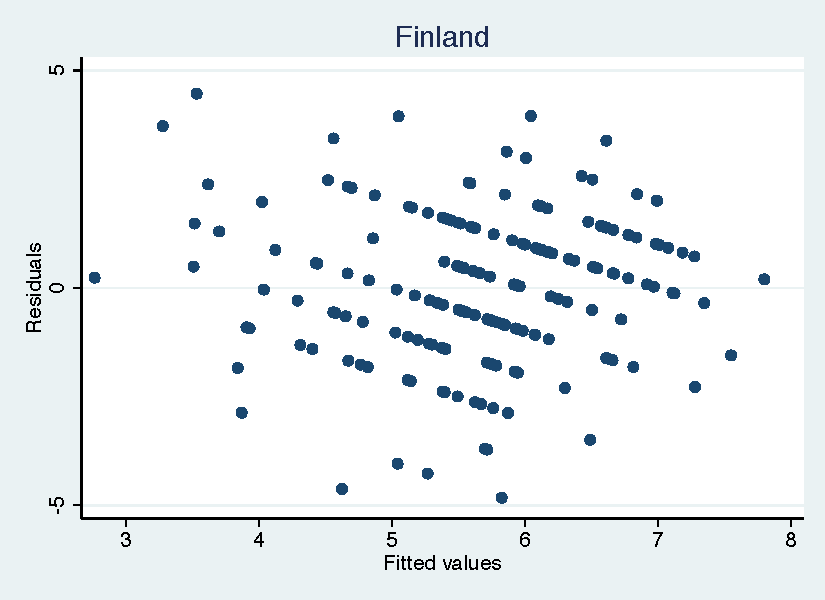
\includegraphics[width=\textwidth]{Residuals/CountryIdeo/Finland}
		\caption{Self-Placement Ideology}
	\end{subfigure}
	\hfill
	\begin{subfigure}[b]{0.475\textwidth}
		\centering 
		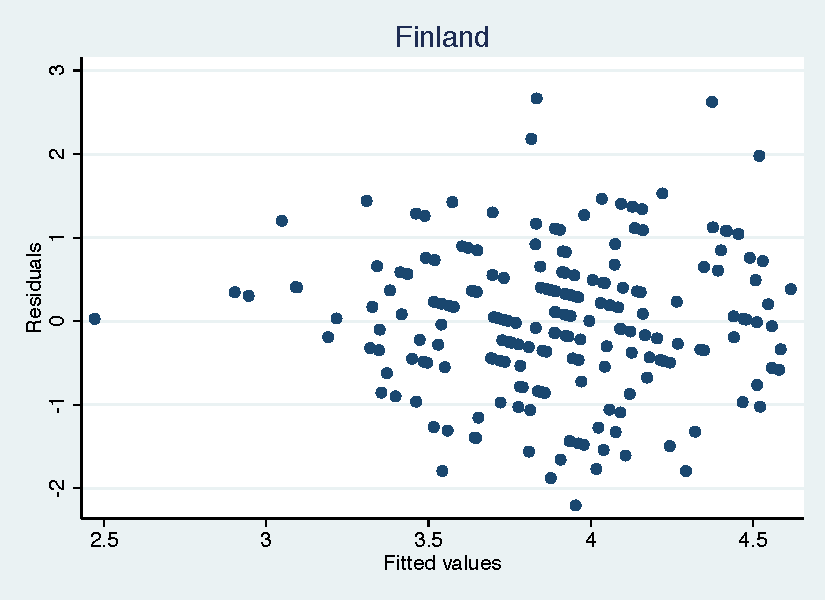
\includegraphics[width=\textwidth]{Residuals/CountryLib/Finland}
		\caption{Issue Stances}
	\end{subfigure}
	\caption{Finland}
	\label{Finland}
\end{figure}

\begin{figure}[H]
	\centering
	\begin{subfigure}[b]{0.475\textwidth}   
		\centering 
		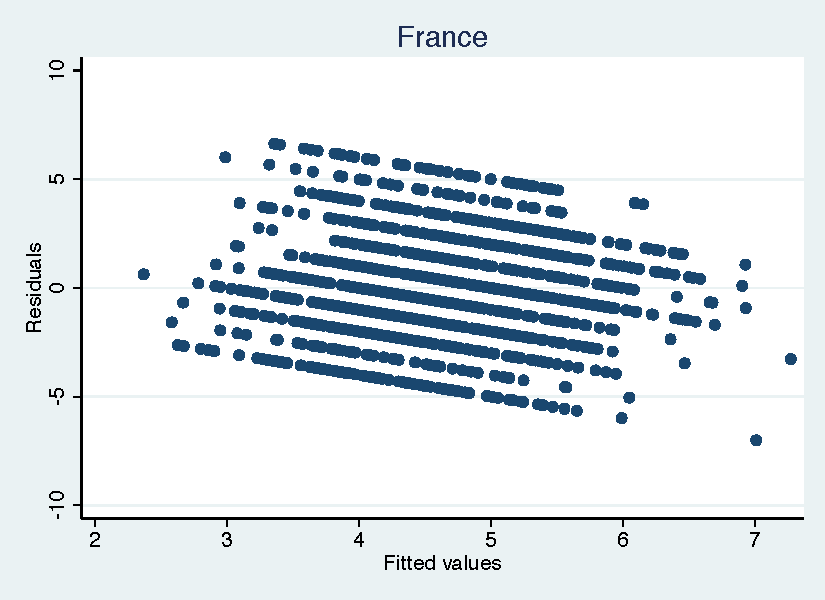
\includegraphics[width=\textwidth]{Residuals/CountryIdeo/France}
		\caption{Self-Placement Ideology}
	\end{subfigure}
	\hfill
	\begin{subfigure}[b]{0.475\textwidth}
		\centering 
		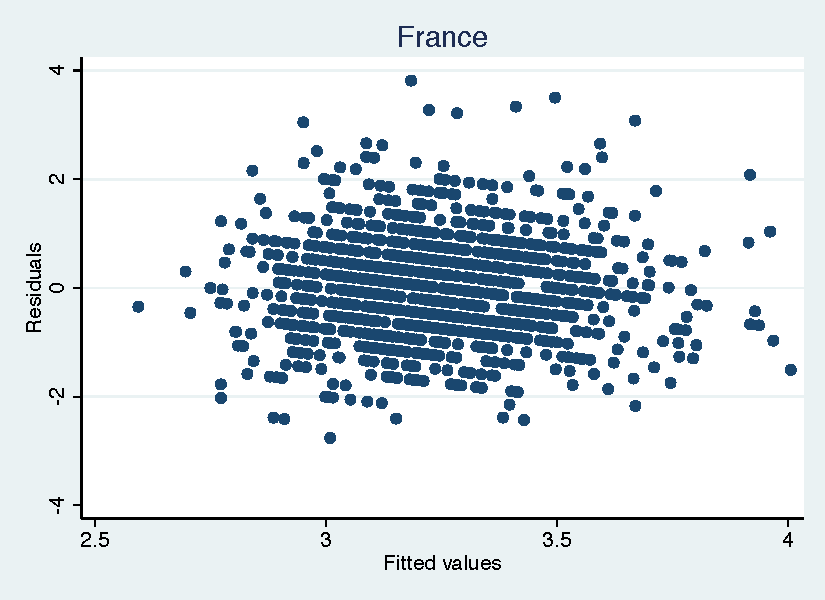
\includegraphics[width=\textwidth]{Residuals/CountryLib/France}
		\caption{Issue Stances}
	\end{subfigure}
	\caption{France}
	\label{France}
\end{figure}

\begin{figure}[H]
	\centering
	\begin{subfigure}[b]{0.475\textwidth}   
		\centering 
		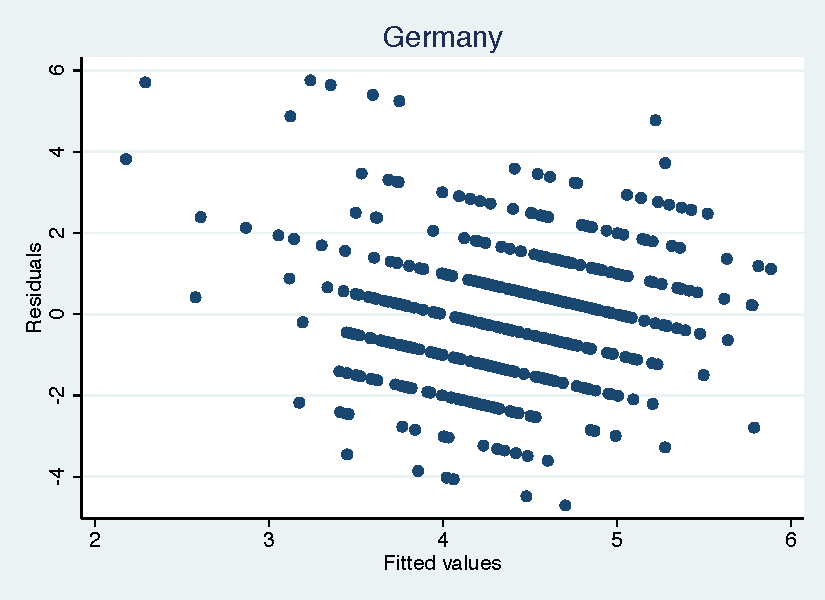
\includegraphics[width=\textwidth]{Residuals/CountryIdeo/Germany}
		\caption{Self-Placement Ideology}
	\end{subfigure}
	\hfill
	\begin{subfigure}[b]{0.475\textwidth}
		\centering 
		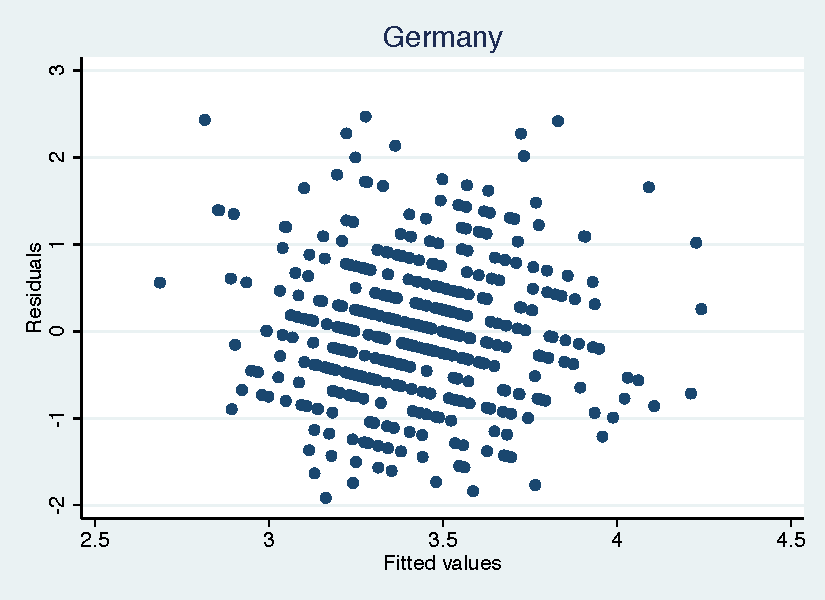
\includegraphics[width=\textwidth]{Residuals/CountryLib/Germany}
		\caption{Issue Stances}
	\end{subfigure}
	\caption{Germany}
	\label{Germany}
\end{figure}

\begin{figure}[H]
	\centering
	\begin{subfigure}[b]{0.475\textwidth}   
		\centering 
		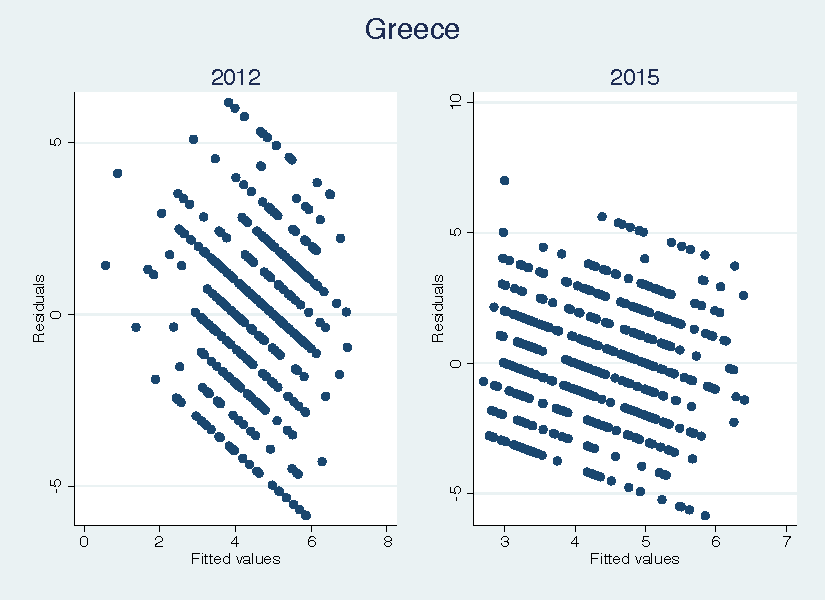
\includegraphics[width=\textwidth]{Residuals/CountryIdeo/Greece}
		\caption{Self-Placement Ideology}
	\end{subfigure}
	\hfill
	\begin{subfigure}[b]{0.475\textwidth}
		\centering 
		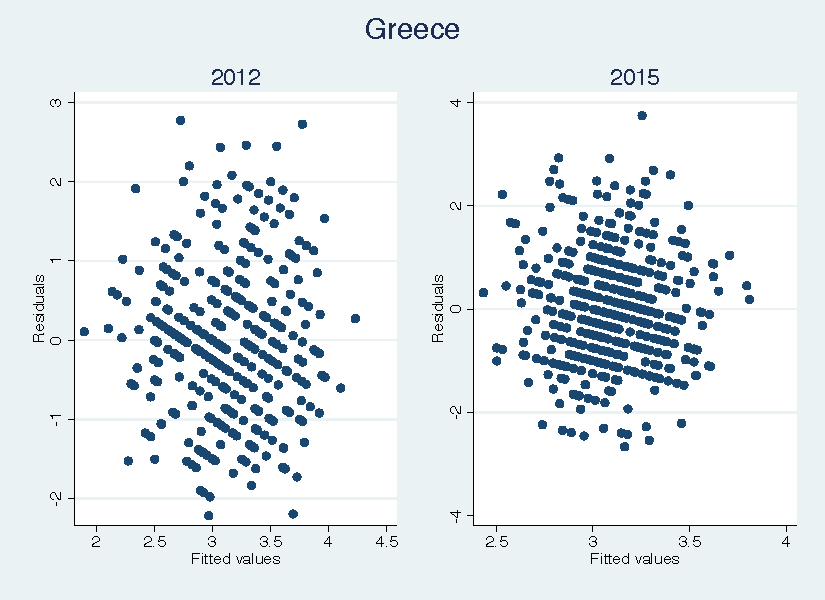
\includegraphics[width=\textwidth]{Residuals/CountryLib/Greece}
		\caption{Issue Stances}
	\end{subfigure}
	\caption{Greece}
	\label{Greece}
\end{figure}

\begin{figure}[H]
	\centering
	\begin{subfigure}[b]{0.475\textwidth}   
		\centering 
		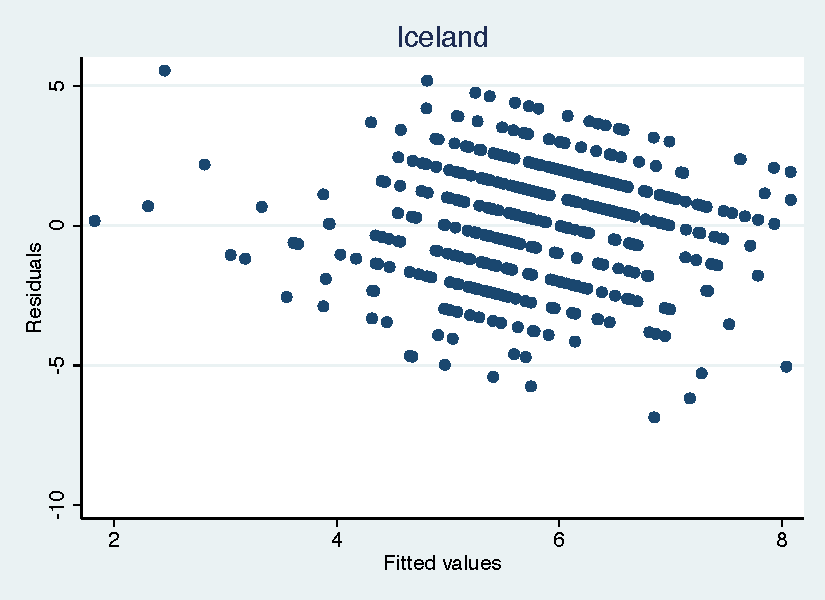
\includegraphics[width=\textwidth]{Residuals/CountryIdeo/Iceland}
		\caption{Self-Placement Ideology}
	\end{subfigure}
	\hfill
	\begin{subfigure}[b]{0.475\textwidth}
		\centering 
		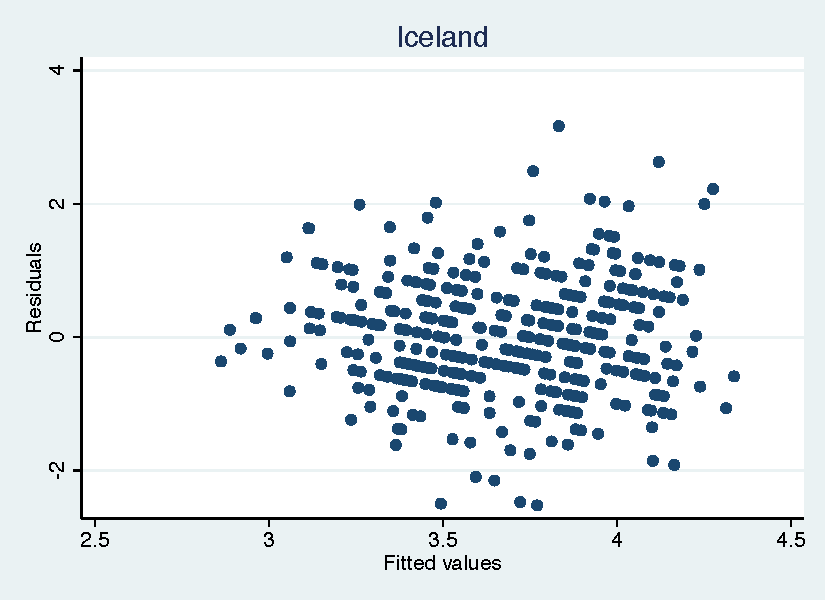
\includegraphics[width=\textwidth]{Residuals/CountryLib/Iceland}
		\caption{Issue Stances}
	\end{subfigure}
	\caption{Iceland}
	\label{Iceland}
\end{figure}

\begin{figure}[H]
	\centering
	\begin{subfigure}[b]{0.475\textwidth}   
		\centering 
		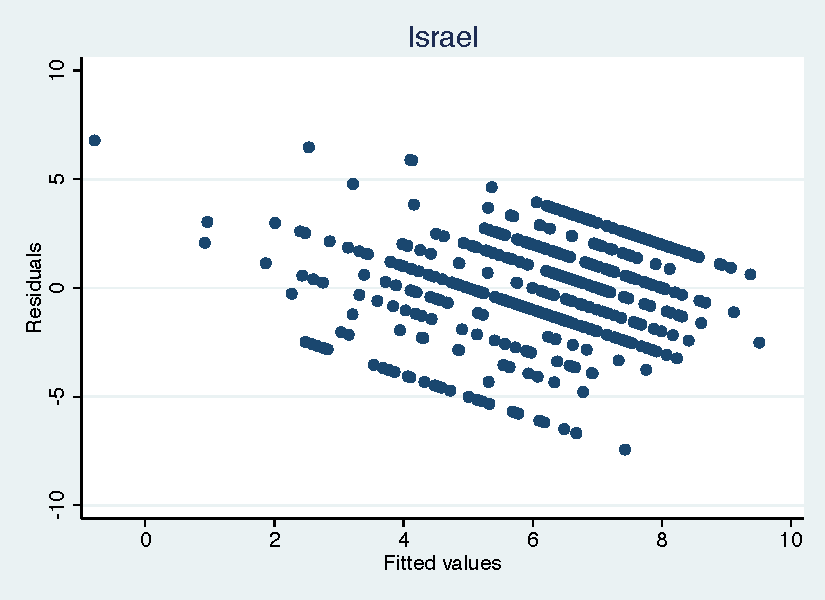
\includegraphics[width=\textwidth]{Residuals/CountryIdeo/Israel}
		\caption{Self-Placement Ideology}
	\end{subfigure}
	\hfill
	\begin{subfigure}[b]{0.475\textwidth}
		\centering 
		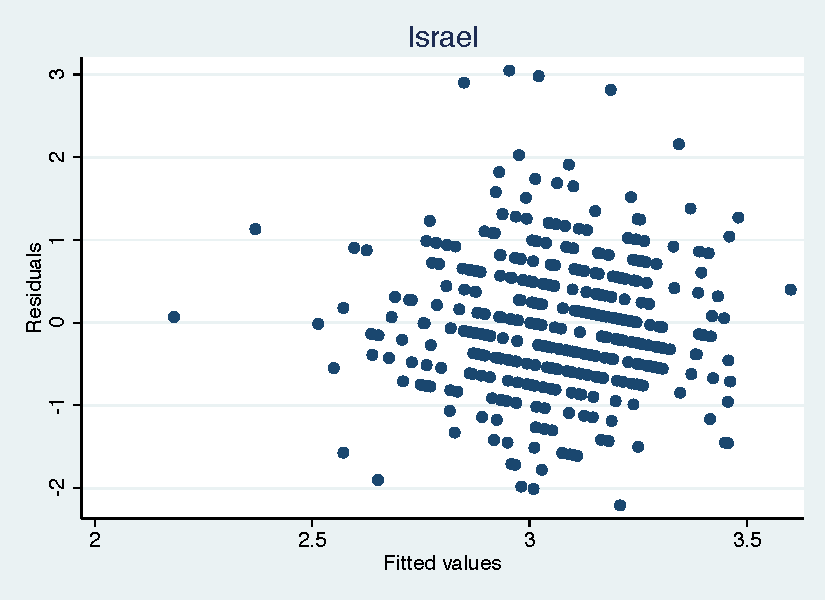
\includegraphics[width=\textwidth]{Residuals/CountryLib/Israel}
		\caption{Issue Stances}
	\end{subfigure}
	\caption{Israel}
	\label{Israel}
\end{figure}

\begin{figure}[H]
	\centering
	\begin{subfigure}[b]{0.475\textwidth}   
		\centering 
		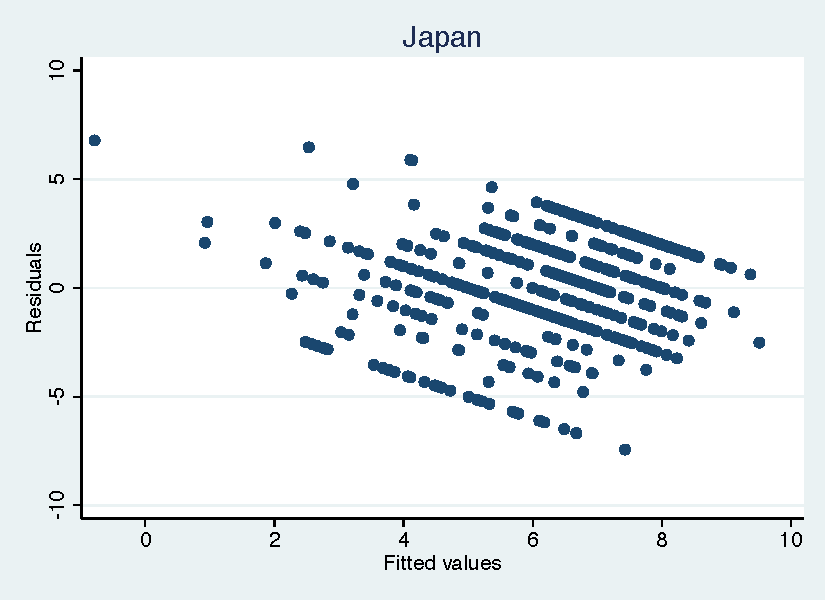
\includegraphics[width=\textwidth]{Residuals/CountryIdeo/Japan}
		\caption{Self-Placement Ideology}
	\end{subfigure}
	\hfill
	\begin{subfigure}[b]{0.475\textwidth}
		\centering 
		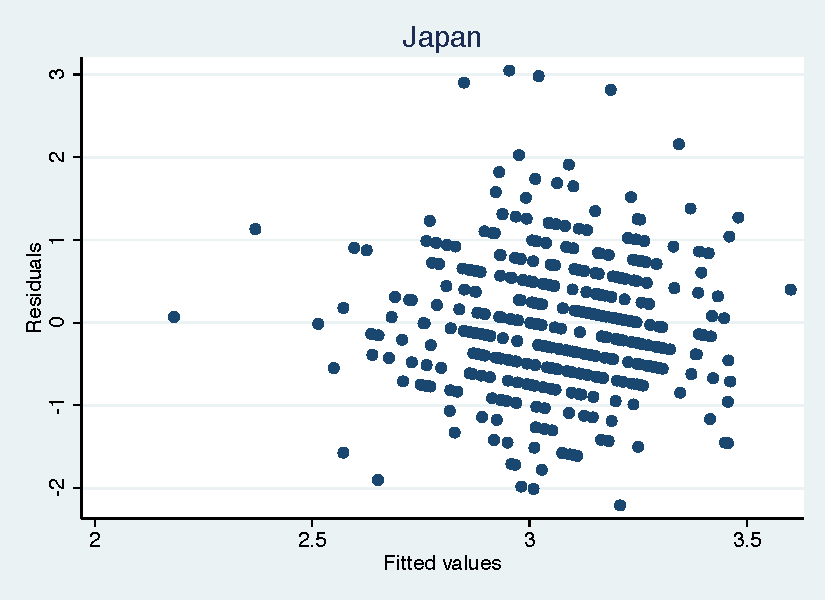
\includegraphics[width=\textwidth]{Residuals/CountryLib/Japan}
		\caption{Issue Stances}
	\end{subfigure}
	\caption{Japan}
	\label{Japan}
\end{figure}

\begin{figure}[H]
	\centering
	\begin{subfigure}[b]{0.475\textwidth}   
		\centering 
		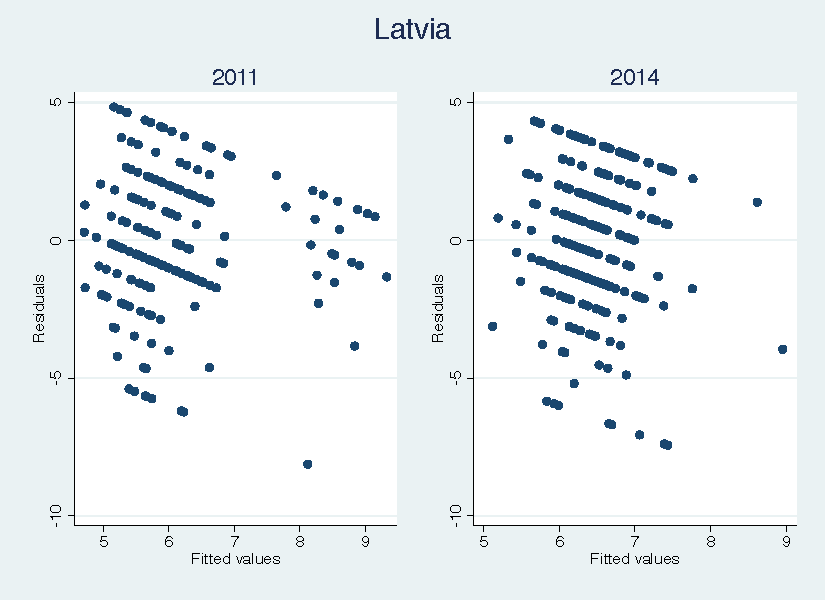
\includegraphics[width=\textwidth]{Residuals/CountryIdeo/Latvia}
		\caption{Self-Placement Ideology}
	\end{subfigure}
	\hfill
	\begin{subfigure}[b]{0.475\textwidth}
		\centering 
		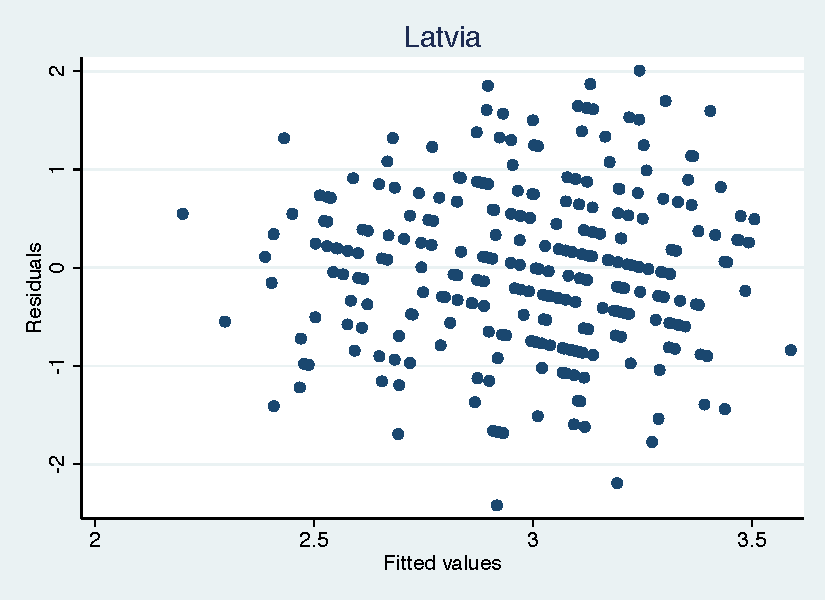
\includegraphics[width=\textwidth]{Residuals/CountryLib/Latvia}
		\caption{Issue Stances}
	\end{subfigure}
	\caption{Latvia}
	\label{Latvia}
\end{figure}

\begin{figure}[H]
	\centering
	\begin{subfigure}[b]{0.475\textwidth}   
		\centering 
		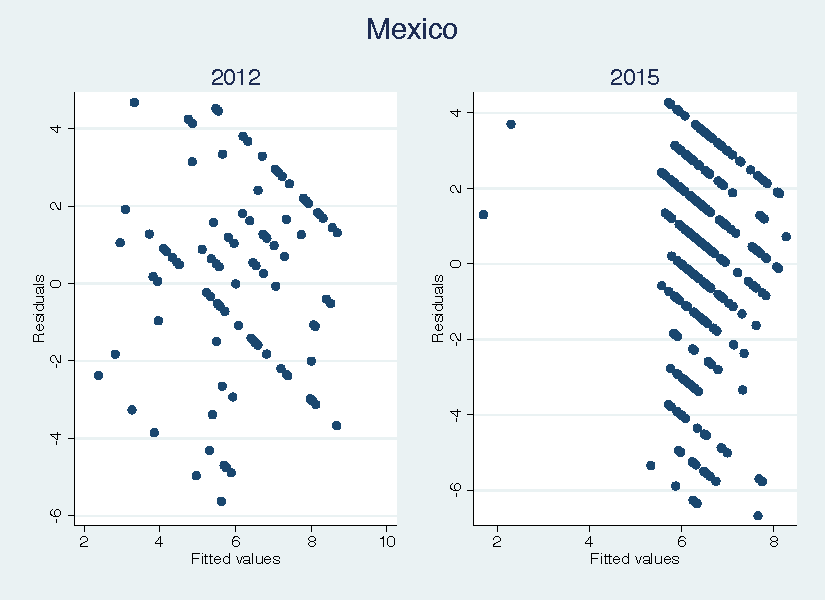
\includegraphics[width=\textwidth]{Residuals/CountryIdeo/Mexico}
		\caption{Self-Placement Ideology}
	\end{subfigure}
	\hfill
	\begin{subfigure}[b]{0.475\textwidth}
		\centering 
		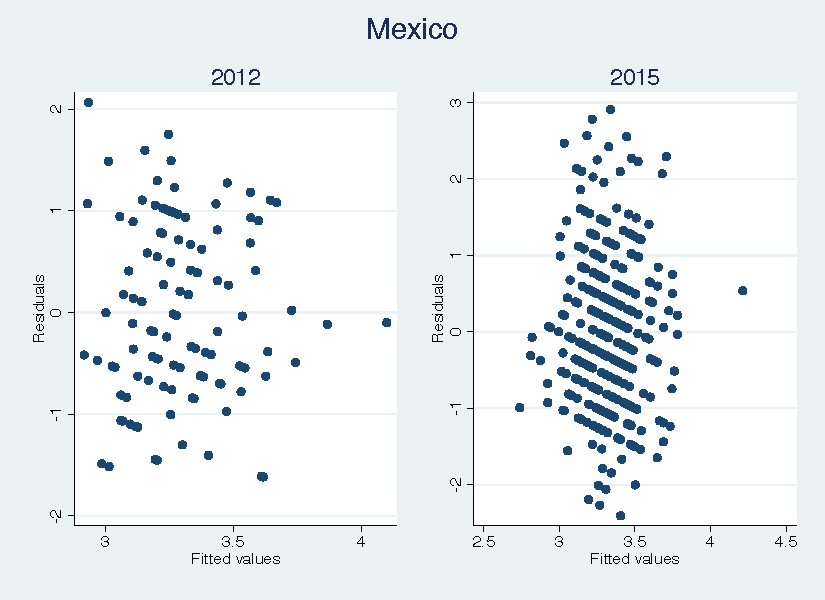
\includegraphics[width=\textwidth]{Residuals/CountryLib/Mexico}
		\caption{Issue Stances}
	\end{subfigure}
	\caption{Mexico}
	\label{Mexico}
\end{figure}

\begin{figure}[H]
	\centering
	\begin{subfigure}[b]{0.475\textwidth}   
		\centering 
		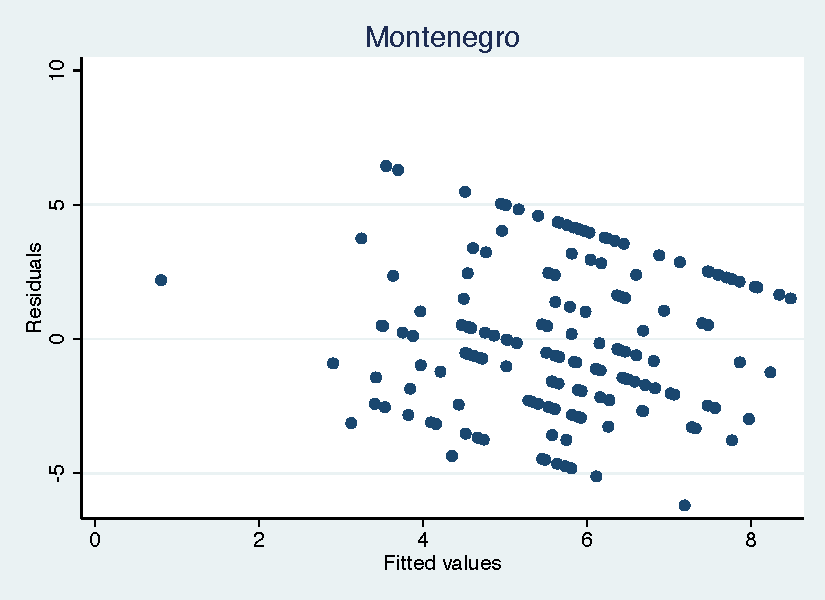
\includegraphics[width=\textwidth]{Residuals/CountryIdeo/Montenegro}
		\caption{Self-Placement Ideology}
	\end{subfigure}
	\hfill
	\begin{subfigure}[b]{0.475\textwidth}
		\centering 
		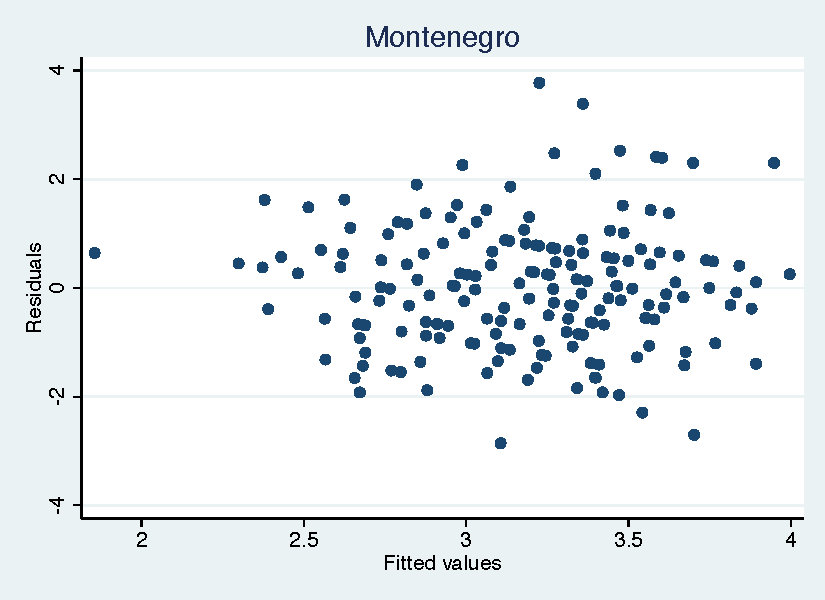
\includegraphics[width=\textwidth]{Residuals/CountryLib/Montenegro}
		\caption{Issue Stances}
	\end{subfigure}
	\caption{Montenegro}
	\label{Montenegro}
\end{figure}

\begin{figure}[H]
	\centering
	\begin{subfigure}[b]{0.475\textwidth}   
		\centering 
		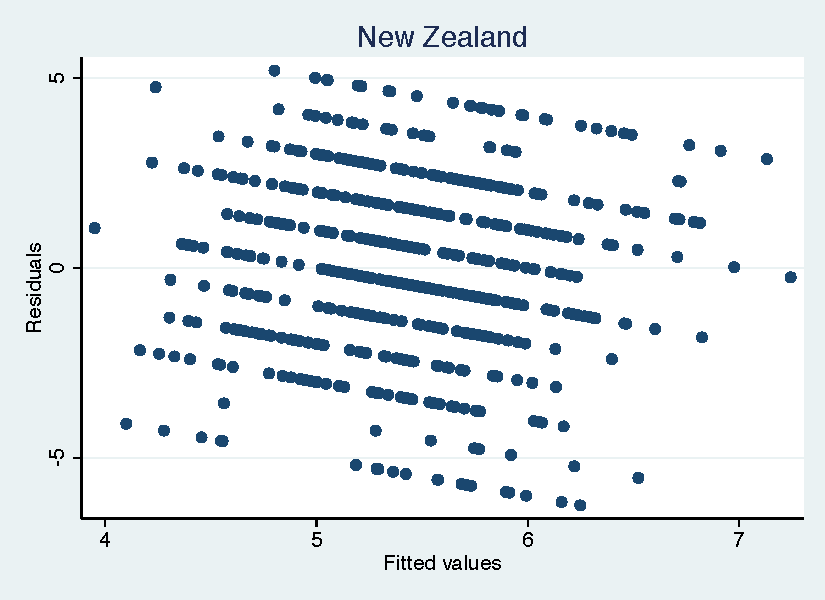
\includegraphics[width=\textwidth]{Residuals/CountryIdeo/NZealand}
		\caption{Self-Placement Ideology}
	\end{subfigure}
	\hfill
	\begin{subfigure}[b]{0.475\textwidth}
		\centering 
		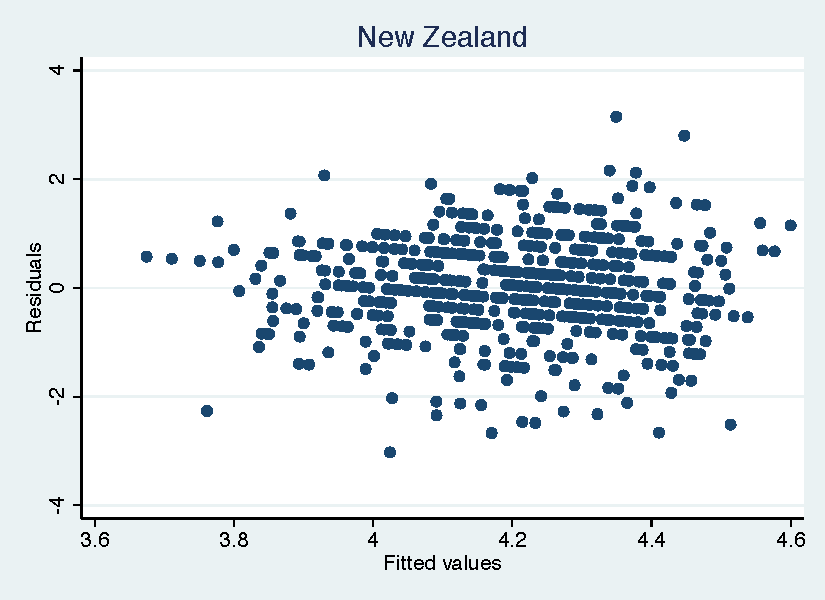
\includegraphics[width=\textwidth]{Residuals/CountryLib/NZealand}
		\caption{Issue Stances}
	\end{subfigure}
	\caption{New Zealand}
	\label{NZealand}
\end{figure}

\begin{figure}[H]
	\centering
	\begin{subfigure}[b]{0.475\textwidth}   
		\centering 
		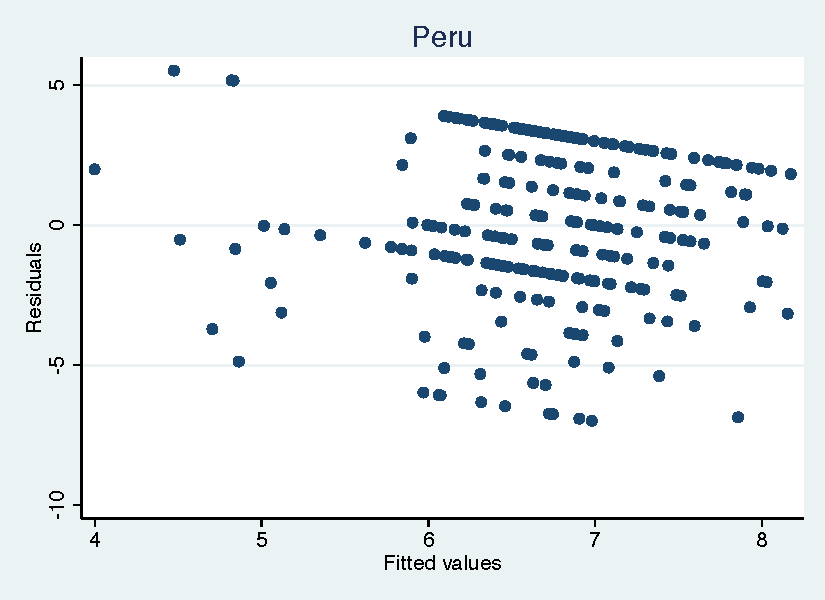
\includegraphics[width=\textwidth]{Residuals/CountryIdeo/Peru}
		\caption{Self-Placement Ideology}
	\end{subfigure}
	\hfill
	\begin{subfigure}[b]{0.475\textwidth}
		\centering 
		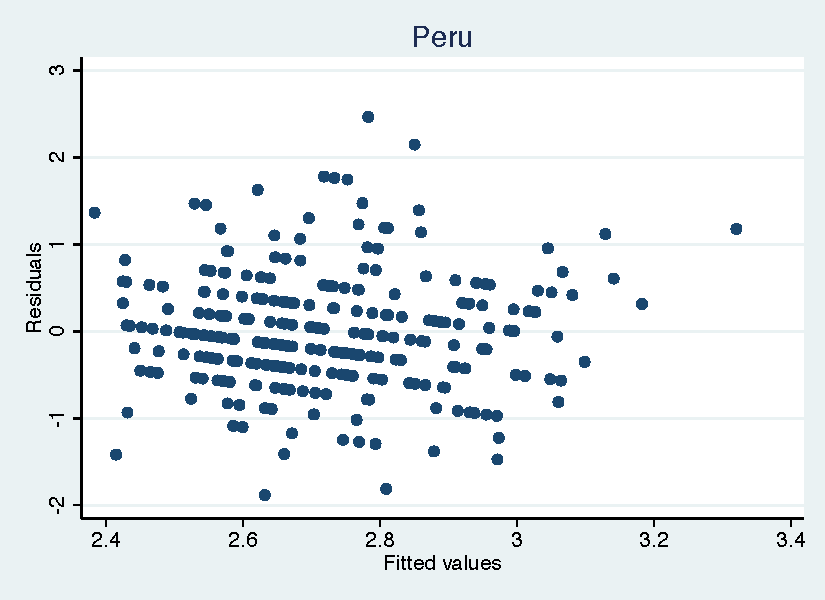
\includegraphics[width=\textwidth]{Residuals/CountryLib/Peru}
		\caption{Issue Stances}
	\end{subfigure}
	\caption{Peru}
	\label{Peru}
\end{figure}

\begin{figure}[H]
	\centering
	\begin{subfigure}[b]{0.475\textwidth}   
		\centering 
		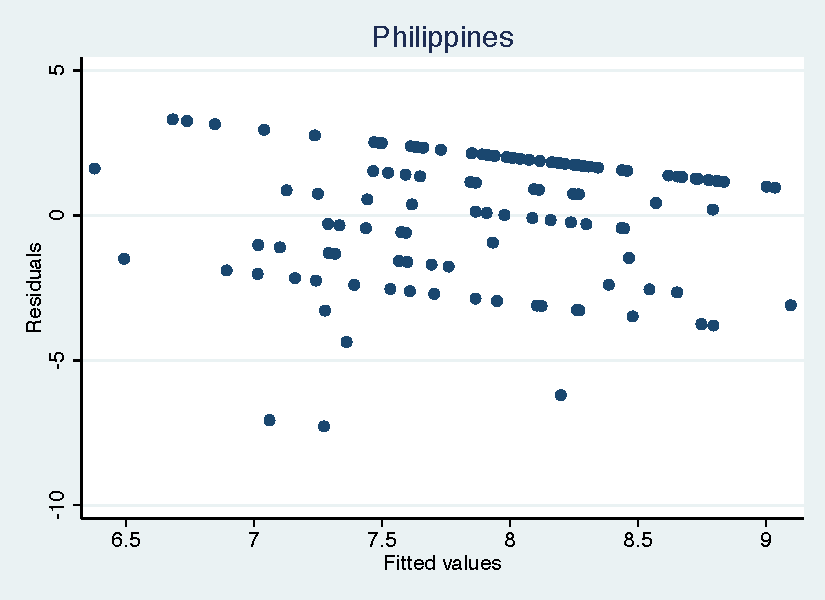
\includegraphics[width=\textwidth]{Residuals/CountryIdeo/Philippines}
		\caption{Self-Placement Ideology}
	\end{subfigure}
	\hfill
	\begin{subfigure}[b]{0.475\textwidth}
		\centering 
		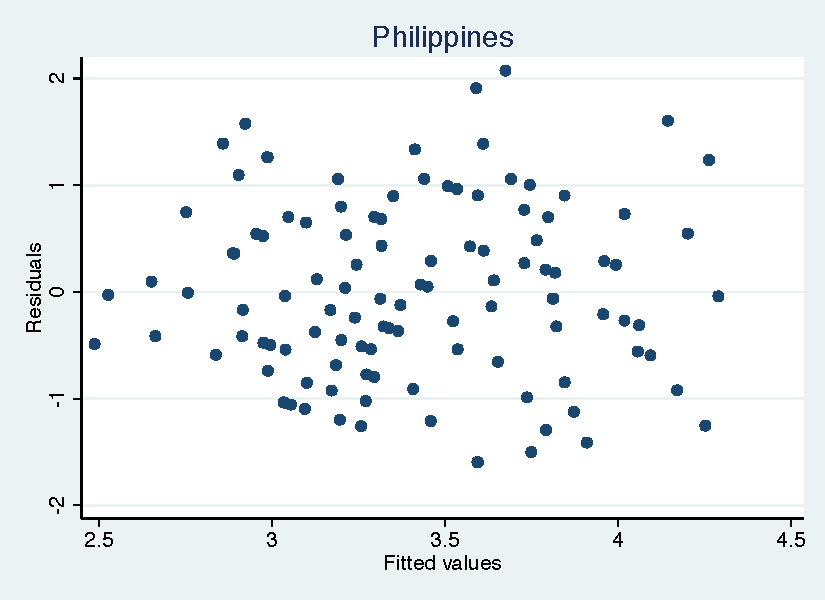
\includegraphics[width=\textwidth]{Residuals/CountryLib/Philippines}
		\caption{Issue Stances}
	\end{subfigure}
	\caption{Philippines}
	\label{Philippines}
\end{figure}

\begin{figure}[H]
	\centering
	\begin{subfigure}[b]{0.475\textwidth}   
		\centering 
		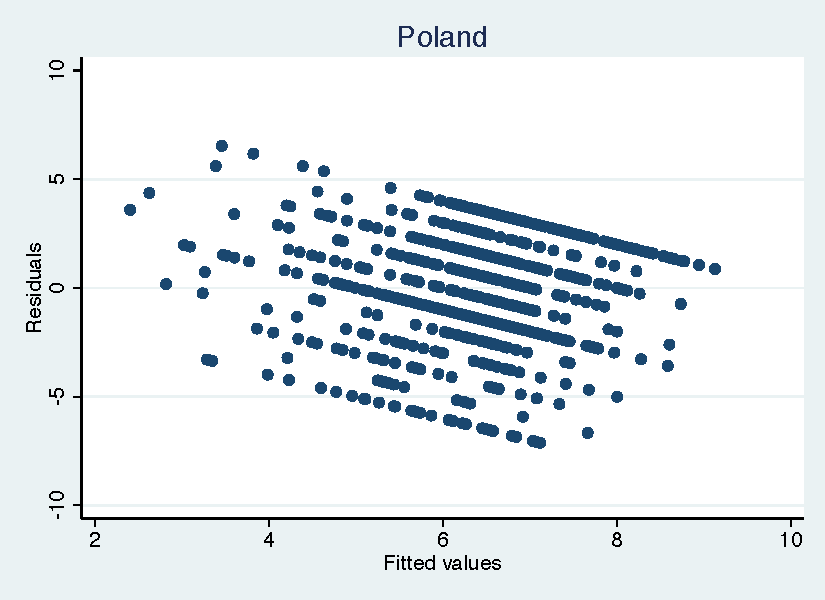
\includegraphics[width=\textwidth]{Residuals/CountryIdeo/Poland}
		\caption{Self-Placement Ideology}
	\end{subfigure}
	\hfill
	\begin{subfigure}[b]{0.475\textwidth}
		\centering 
		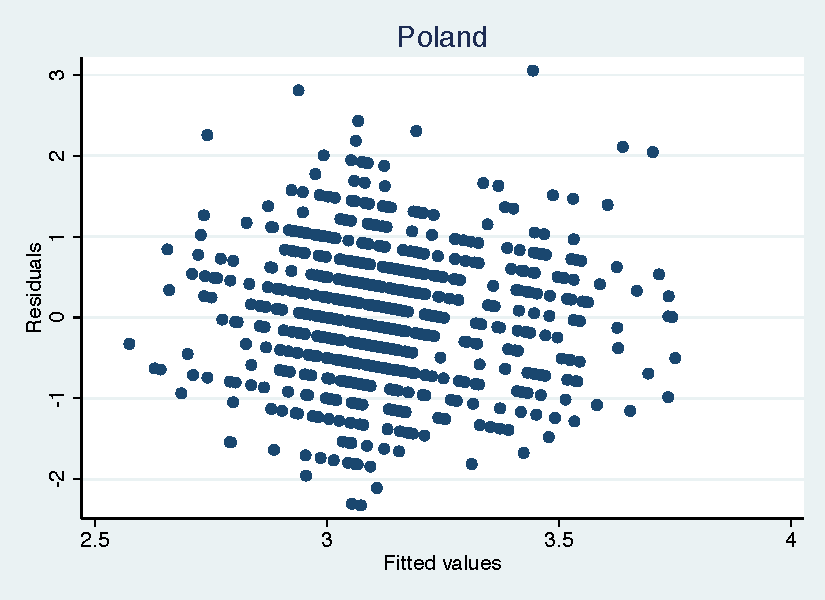
\includegraphics[width=\textwidth]{Residuals/CountryLib/Poland}
		\caption{Issue Stances}
	\end{subfigure}
	\caption{Poland}
	\label{Poland}
\end{figure}

\begin{figure}[H]
	\centering
	\begin{subfigure}[b]{0.475\textwidth}   
		\centering 
		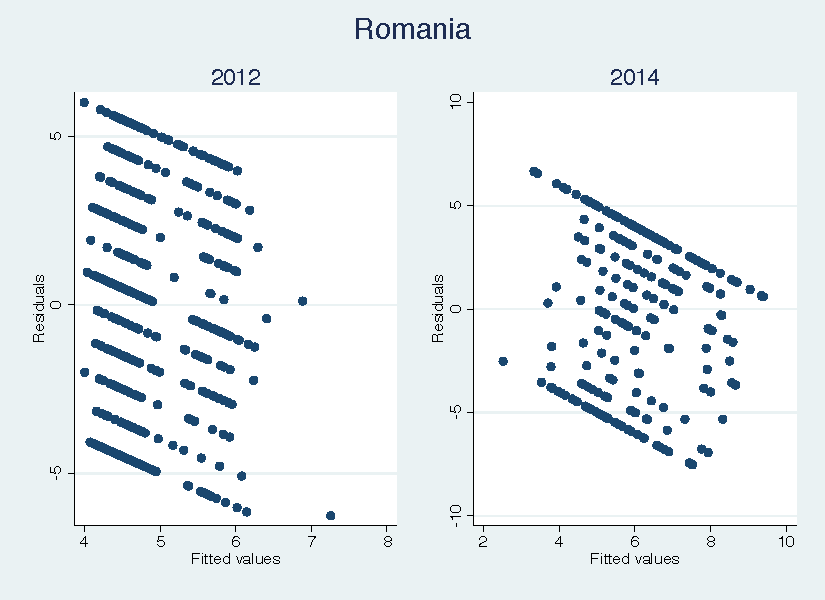
\includegraphics[width=\textwidth]{Residuals/CountryIdeo/Romania}
		\caption{Self-Placement Ideology}
	\end{subfigure}
	\hfill
	\begin{subfigure}[b]{0.475\textwidth}
		\centering 
		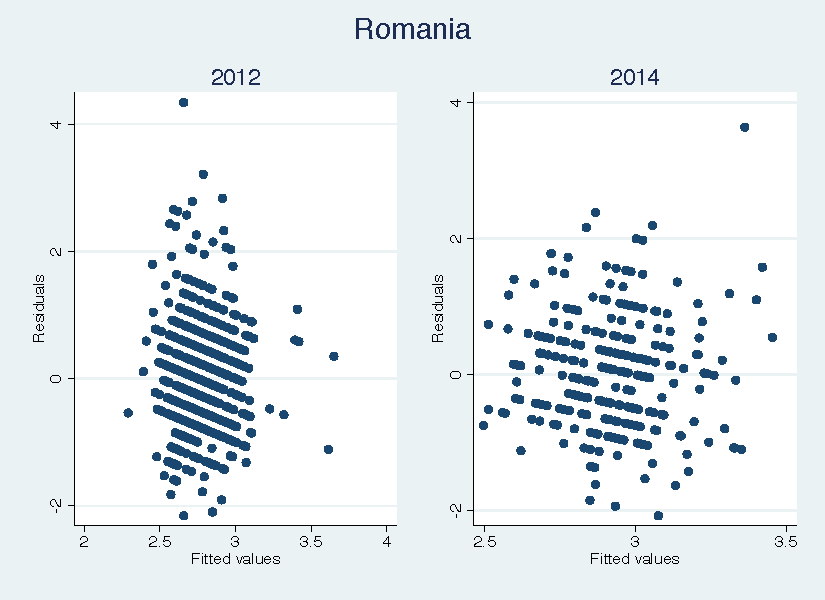
\includegraphics[width=\textwidth]{Residuals/CountryLib/Romania}
		\caption{Issue Stances}
	\end{subfigure}
	\caption{Romania}
	\label{Romania}
\end{figure}

\begin{figure}[H]
	\centering 
	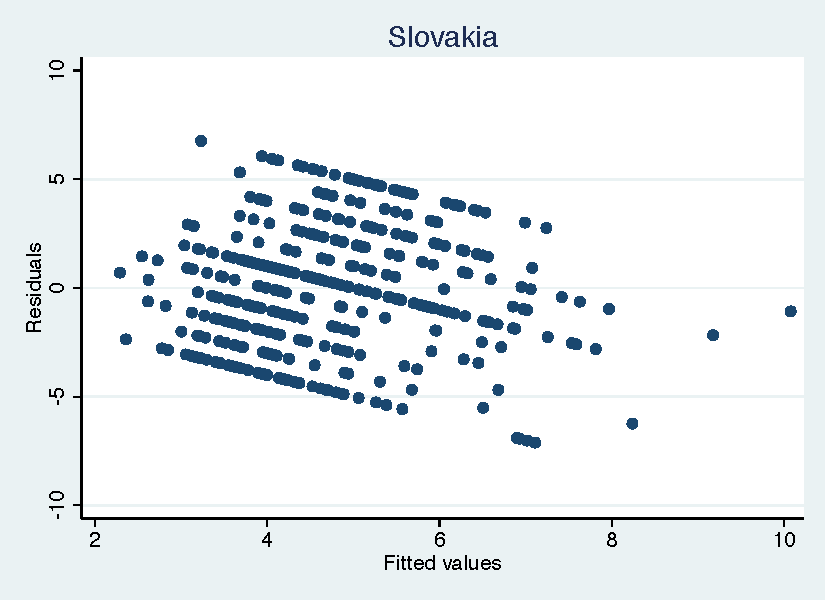
\includegraphics[width=\textwidth]{Residuals/CountryIdeo/Slovakia}
	\caption{Slovakia - Self-Placement Ideology}
	\label{Slovakia}
\end{figure}

\begin{figure}[H]
	\centering
	\begin{subfigure}[b]{0.475\textwidth}   
		\centering 
		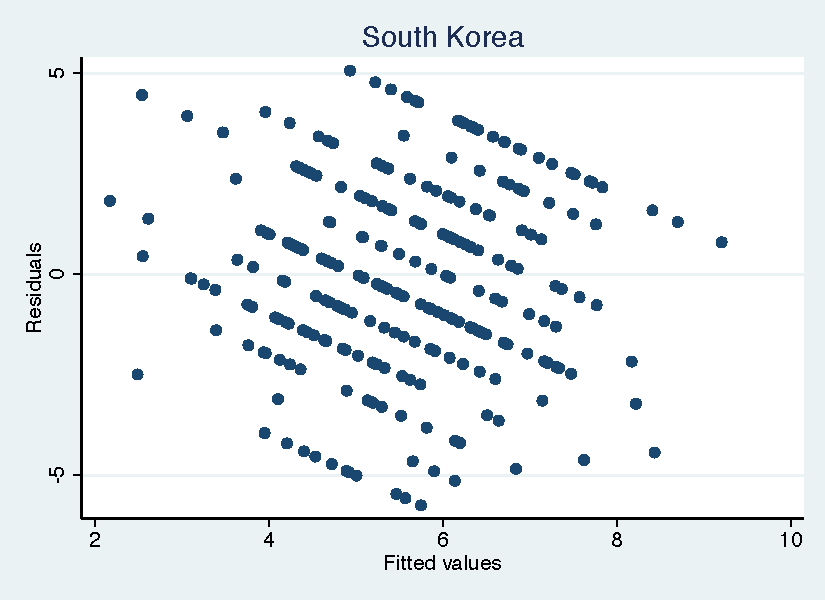
\includegraphics[width=\textwidth]{Residuals/CountryIdeo/SKorea}
		\caption{Self-Placement Ideology}
	\end{subfigure}
	\hfill
	\begin{subfigure}[b]{0.475\textwidth}
		\centering 
		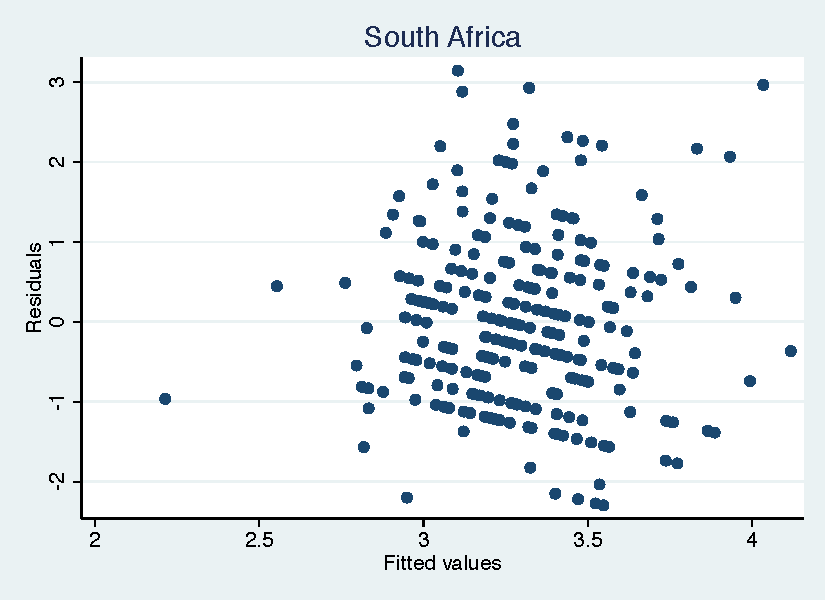
\includegraphics[width=\textwidth]{Residuals/CountryLib/SAfrica}
		\caption{Issue Stances}
	\end{subfigure}
	\caption{South Africa}
	\label{SAfrica}
\end{figure}

\begin{figure}[H]
	\centering
	\begin{subfigure}[b]{0.475\textwidth}   
		\centering 
		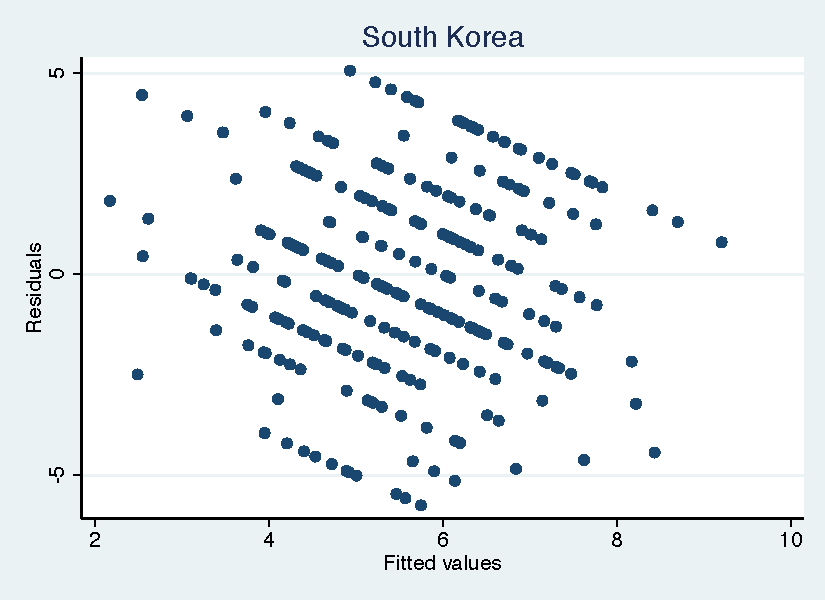
\includegraphics[width=\textwidth]{Residuals/CountryIdeo/SKorea}
		\caption{Self-Placement Ideology}
	\end{subfigure}
	\hfill
	\begin{subfigure}[b]{0.475\textwidth}
		\centering 
		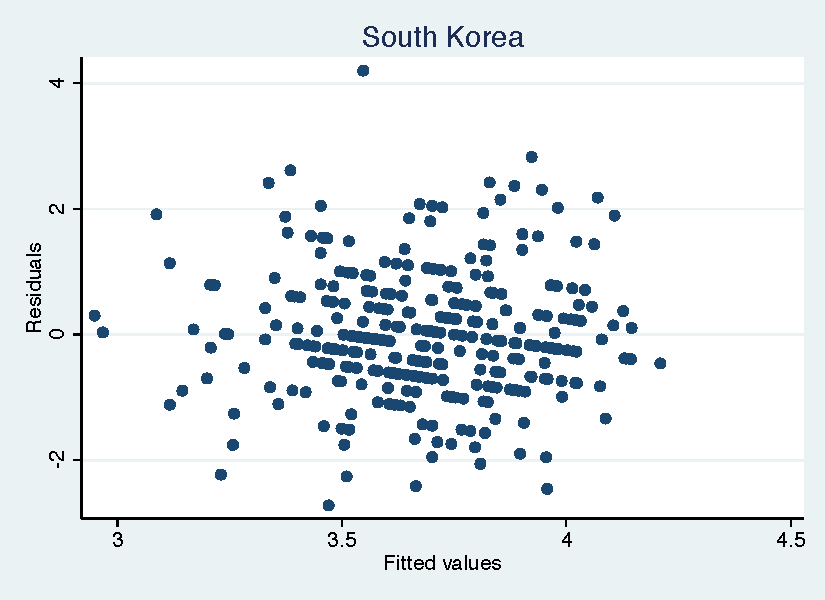
\includegraphics[width=\textwidth]{Residuals/CountryLib/SKorea}
		\caption{Issue Stances}
	\end{subfigure}
	\caption{South Korea}
	\label{SKorea}
\end{figure}

\begin{figure}[H]
	\centering
	\begin{subfigure}[b]{0.475\textwidth}   
		\centering 
		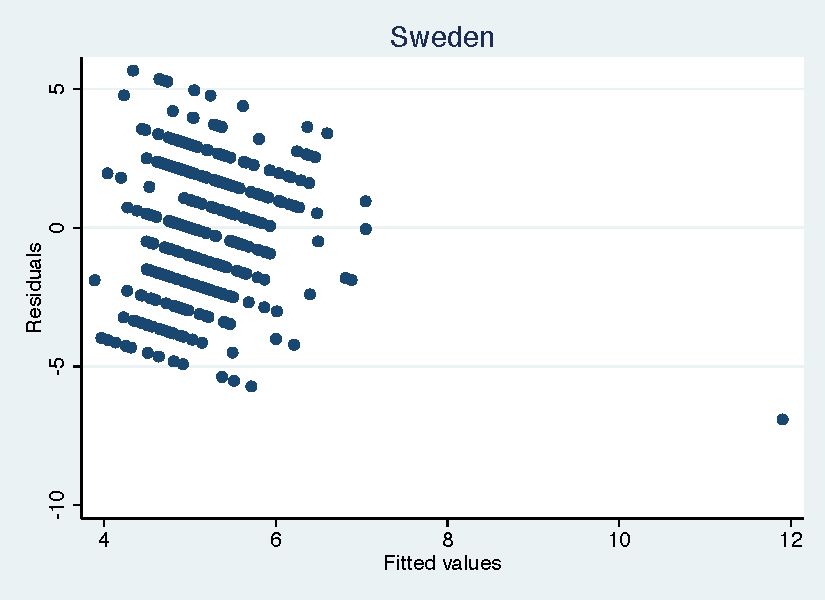
\includegraphics[width=\textwidth]{Residuals/CountryIdeo/Sweden}
		\caption{Self-Placement Ideology}
	\end{subfigure}
	\hfill
	\begin{subfigure}[b]{0.475\textwidth}
		\centering 
		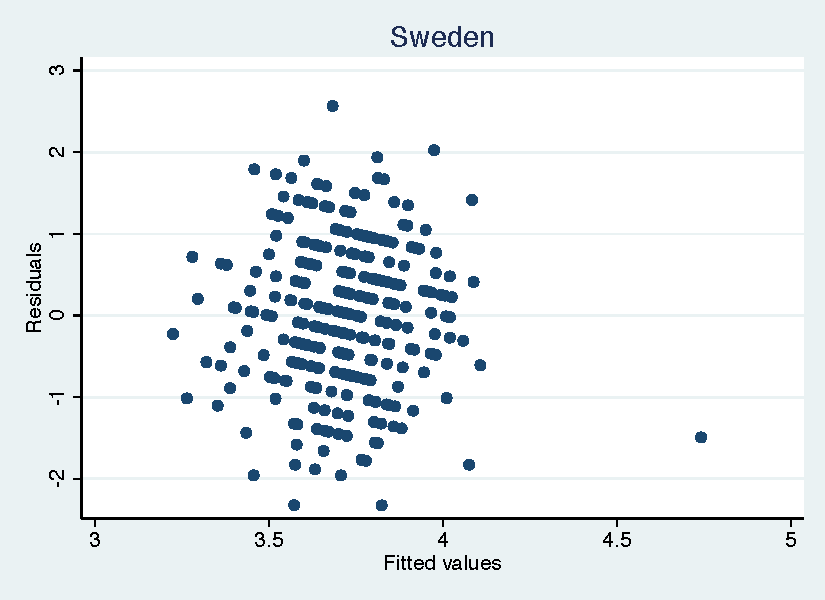
\includegraphics[width=\textwidth]{Residuals/CountryLib/Sweden}
		\caption{Issue Stances}
	\end{subfigure}
	\caption{Sweden}
	\label{Sweden}
\end{figure}

\begin{figure}[H]
	\centering
	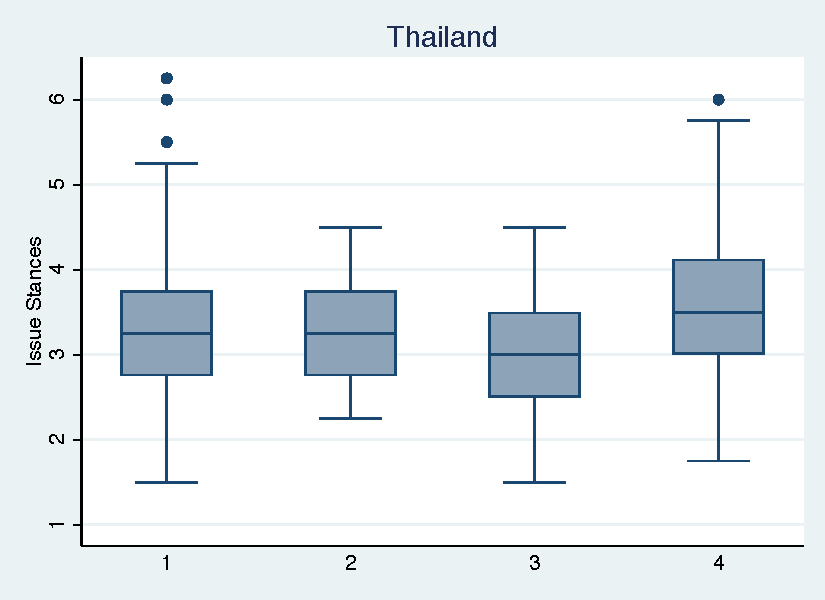
\includegraphics[width=\textwidth]{Residuals/CountryLib/Thailand}
	\caption{Thailand - Issue Stances}
	\label{Thailand}
\end{figure}

\begin{figure}[H]
	\centering
	\begin{subfigure}[b]{0.475\textwidth}   
		\centering 
		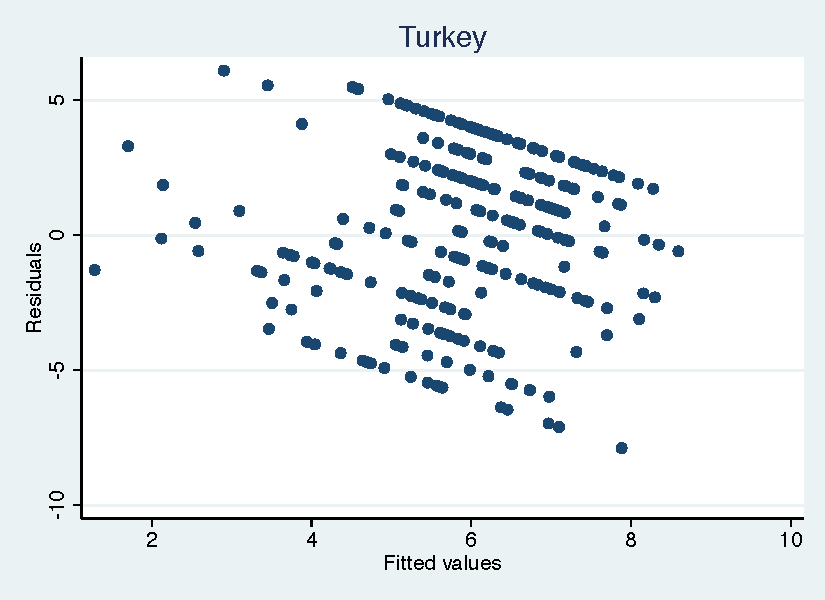
\includegraphics[width=\textwidth]{Residuals/CountryIdeo/Turkey}
		\caption{Self-Placement Ideology}
	\end{subfigure}
	\hfill
	\begin{subfigure}[b]{0.475\textwidth}
		\centering 
		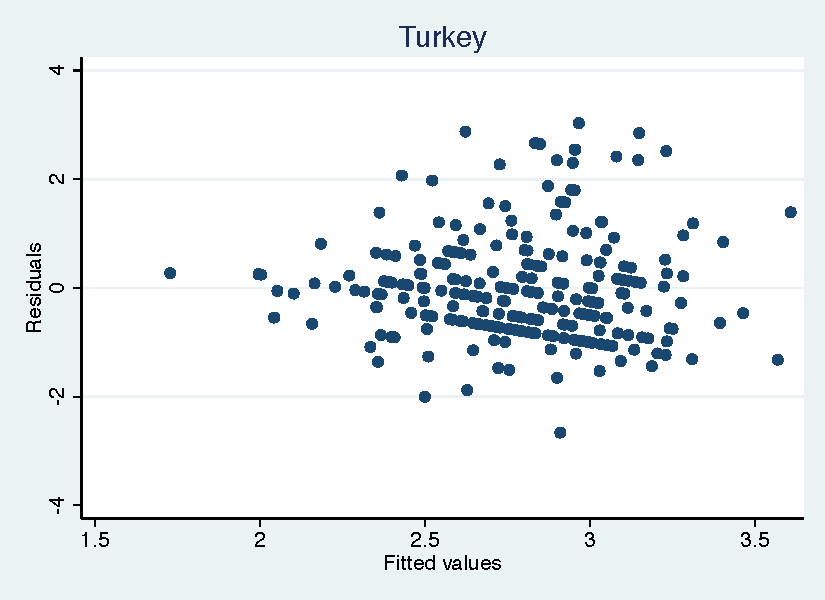
\includegraphics[width=\textwidth]{Residuals/CountryLib/Turkey}
		\caption{Issue Stances}
	\end{subfigure}
	\caption{Turkey}
	\label{Turkey}
\end{figure}

\end{document}